\documentclass{article}
\title{Math 425 Assignment 2}
\author{Max Horowitz-Gelb}
\date{October 30, 2016}
\usepackage{graphicx}
\usepackage{amsmath}
\DeclareMathOperator*{\argmin}{argmin}

\setlength{\parindent}{0pt}
\setlength{\parskip}{10pt}

\begin{document}
\maketitle
\section*{Teammate}
Tushar Verma was originally a partner on this assignment
but has chosen to drop the course. Due to the lack of time
to find a new partner, the instructor has permitted this assignment to be completed by me solely.

\section*{Problem 1}
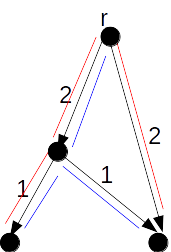
\includegraphics[scale=0.5]{tree}

In this figure a minimum spanning tree rooted at $r$ is labeled with blue lines and a tree created from a set of least cost dipaths from $r$ is labeled with red lines. These two trees are clearly different from eachother. As one can see the MST does not contain all least cost dipaths since the cost from $r$ to the bottom right node is of cost 3 and there is a cheaper dipath of cost 2. Conversely the cost of the tree made from the minimum cost dipaths is of cost 5 but the MST is of cost 4, therefore the minimum dipath tree is not an MST.
\section*{Problem 2}
Given a digraph $G = (V,E)$, costs $c_e$ for every $e \in E$ and disjoint sets $R,S \subset V$. Then the problem of finding a least cost dipath starting from any node in $R$ and ending in any node in $S$ can be reduced to solving one ordinary shortest path problem by lightly modifying $G$. Simply make a new graph by adding a special node $\gamma$ to $V$ and arcs from $\gamma$ to all nodes in $R$, all with cost $0$. Call this new graph  $G'$.

If G has no negative cost dicircuits, then if we run ordinary least cost dipaths on $G'$ with $r = \gamma$ and achieve a feasible potential $y$ and least cost dipaths
described by 
$p$, our least cost dipath from $R$ to $S$ in $G$ is a dipath that ends in $t = \argmin\limits_{v \in S} y_v$. Its cost is $y_t$ and its dipath is the dipath in $p$ ending with $t$ with node $\gamma$ and outgoing arcs from $\gamma$ removed.

First note that $G$ has no negative cost dicircuits if and only if $G'$ has none since $\gamma$ has only outgoing arcs and therefore cannot be part of a circuit.

Now we shall prove this is a valid reduction via contradiction. Assume that there exists a dipath, $x$, from node $a \in R$ to $b \in S$ in $G$ with less cost than any dipath found from ordinary least cost dipaths on $G'$ with $r=\gamma$. Since there is a 0 cost arc from $\gamma$ to $a$ then $y_a \leq 0$. Then if the cost of $x$ is less than all dipaths found in $G'$ then the cost of $x$ is less than $y_b$. But since $x$ exists in $G'$, we could achieve a path from $\gamma$ to $b$ of cost $y_a + cost(x)$ which is less than $y_b$. This creates a contradiction. Therefore the minimum cost dipath from $\gamma$ to $S$ has a cost less than or equal to the least cost dipath from $R$ to $S$ in $G$. 

And since $\gamma$ has only outgoing arcs of cost $0$ then the least cost dipath from $\gamma$ to $S$ must be the same cost as the least cost dipath from $R$ to $S$ in $G$. So by removing $\gamma$ from this path, we obtain a least cost dipath from $R$ to $S$ in $G$.



Finally if $G$ had a negative cost dicircuit then so would $G'$ and running ordinary least cost dipaths on $G'$ would discover this. This would imply there is no solution to the problem.
 
\section*{Problem 3}
Suppose that we are give a shortest dipath problem on a digraph $G$ such that a node $w\neq r$ is incident with two arcs $a$ and $b$. Then we can answer the problem with a smaller digraph in three different ways. 

First note that without loss of generality we may assume there exists a dipath from $r$ to $v$ for all $v \in V$, since if this were not the case for some $v$ then we could add an arc $rv$ with cost $\sum_E |c_e|$. This arc would never be used in any least cost dipath from $r$ to $x \neq v$.

\subsection*{Case 1}
If $w$ has only outgoing arcs, then clearly there is no dipath from $r$ to $w$, and as well any least cost dipath from $r$ to $v$ where $v \neq w$ cannot contain $w$. Hence we can solve the shortest dipath problem on $G$ with $w$ and its incident arcs removed and then simply set $y_w = \inf$ and $p(w) = -1$. 

\subsection*{Case 2}
If $w$ has only incoming arcs, then clearly there is no dipath from $r$ to $v$ where $v \neq w$ and $w$ is in the dipath. Therefore we can do ordinary least cost dipaths on a graph with $w$ and its incident arcs removed to get a $y$ and $p$ such that $p$ will contain the least cost dipath from $r$ to $v$ for all $v \in V \setminus \{w\}$. These least cost dipaths will also be least cost dipaths in the original graph.

Then let $a = \alpha w$ and $b = \beta w$ where $\alpha$ and $\beta$ are two unique nodes in the graph adjacent to $w$. Then assuming we don't find a negative dicircuit in the smaller graph, then since $a$ and $b$ are the only two incoming arcs for $w$ then the last arc in a dipath from $r$ to $w$ must be one of these two arcs. And to minimize the cost of a dipath from $r$ to $w$ it must then contain the minimum dipath from $r$ to $\beta$ or $r$ to $\alpha$. So we set $y_w = min \{ y_\beta + c_b, y_\alpha + c_a\} $ and
$p(w) = v$ such that $(v,e) \in \{(\alpha,a), (\beta,b)\}$ and $y_w = y_v + c_e$.

\subsection*{Case 3}
If $w$ has one incoming arc and one outgoing arc, then we can remove parts of the graph to solve a smaller problem. Let $a = \alpha w$ and let $b = w \beta$ and let $f$ be an arc from $\alpha$ to $\beta$. 


Then there are 3 cases.

\subsubsection*{Case 3a}
$f$ does not exist. 

In this case we can add an arc $f'=\alpha \beta$ of cost $c_a + c_b$ and remove $w$ and its incident arcs from the graph. If there was any least cost dipath from $r$ to any node other than $w$ that contained $w$ in in it, then the part of the dipath containing $w$ would have to be of the form $a, w, b$. Then replacing $a, w, b$ with $f'$ would result in another dipath of same cost. Then we could run ordinary least cost dipaths on our transformed graph to get $y$ and $p$. Since as we've shown, our transformation could not affect the cost of any least cost dipath, then we may simply check if $p(\beta) = \alpha$ and if so set $p(\beta) = w$. Then set $p(w) = \alpha$ and $y_w = y_\alpha + c_a$. This would give us our solution.

\subsubsection*{Case 3a}
$c_f > c_a + c_b$. 

In this case any least cost dipath would never include $f$ since we could simply replace $f$ with $a, w, b$ and
achieve a lower cost. Therefore we can remove $f$ and run ordinary least cost dipaths on the subgraph to get the final solution.



\subsubsection*{Case 3b}
$c_f \leq c_a + c+b$

In this case we can remove the arc $b$ and run ordinary least cost dipath. This is because if $b$ was used in a least cost dipath then so was $a$ and we could replace $a$ and $b$ with $f$ to get a dipath of less than or equal cost. This result would give us a final solution.

\subsection*{Efficiency}
Since all there are a constant number of steps in the reduction, the reduction is $O(1)$


\end{document}

